\section{Field Study}
\label{chapter:field-study}


	The field study took place during the first two weeks of March, from 3/3/2015 to 3/15/2015 in Oettingenstrasse 67, a faculty building of Ludwig-Maximilians-Universit\"at M\"unchen. Data was collected from the display setup on 14 consecutive days and 28 semi-structured interviews were carried out on five working days during the same two weeks. A total of 117 interactions were registered with the public display installation and 57 survey responses were recorded.
	The goal of this study was to test our research questions, and to see how users respond to questionnaires conducted on public displays. We chose to carry out a descriptive study, with a focus on ecological validity, since the research prototype was still in an early stage at this point.




\subsection{Research Questions}

	% MOTIVATE: Why did we bother to do this study?
	One of the main reasons why we conducted this field study, was to get a better understanding of our assumptions and to see how users react to questionnaires on displays in public settings. Besides, it was of importance to conduct a study ``in the wild'', because there often is a discrepancy between lab studies and field studies. This phenomenon was discussed by Ojala and Kostakos in 2011: ``The first important conclusion we have arrived at, [sic] is that there exists a huge difference between results obtained in a lab and in the wild using the exact same configuration''\cite{Ojala2011}.

	% What do we assume  /  What do we want to know
	One hypothesis we made for the development of our first research prototype of the \textit{PDSurvey} platform was that we can simplify the process of conducting and deploying surveys to large public display networks. Since this is a rather large claim, we broke down this hypothesis to the following more fine-grained statements:

	\begin{enumerate}
		\item Which feedback channels are best suited for completing surveys in public?
		\item Why did users approach the display? What motivates them to fill in surveys in public? 
		\item How did the user notice and perceive the survey on the display?
	\end{enumerate}

	In addition to these questions we were also interested in user stories, the feedback real-world users gave us in regards to answering surveys on screens in public. For this reason we also conducted semi-structured interviews in parallel to the quantitative evaluation of the \textit{PDSurvey} platform. In order to get as authentic and personal feedback as possible, we stuck loosely to the designated questions of the semi-structured interview (see Appendix \ref{appendix:interviews}), in order to allow users to also tell us stories about areas which we had not thought of before.
	These research questions influenced the questionnaire we deployed using \textit{PDSurvey} and the questions we asked in the semi-structured interviews. Questions which go beyond the scope of this thesis, and might serve as follow-up questions for further research, are gathered in chapter \ref{chapter:future-work}, Future Work.




% \clearpage
\subsection{Pre-Study}

	Before starting the field study, multiple small pre-studies were made with fellow students and research staff at the chair for Media Informatics. We wanted to get early feedback in the development process for \textit{PDSurvey}. 
	% Backend
	For PDAdmin findings include providing a suitable entry point, general comments regarding how to improve layout and user flow, and to offer a Wizard for beginners. For the admin interface it turned out to be important to reduce all available features to a minimalistic interface, even though the platform is designed to support a wide variety of options. 

	% Figure PDClient Welcome Screen
	\begin{figure}
	    \begin{center}
	        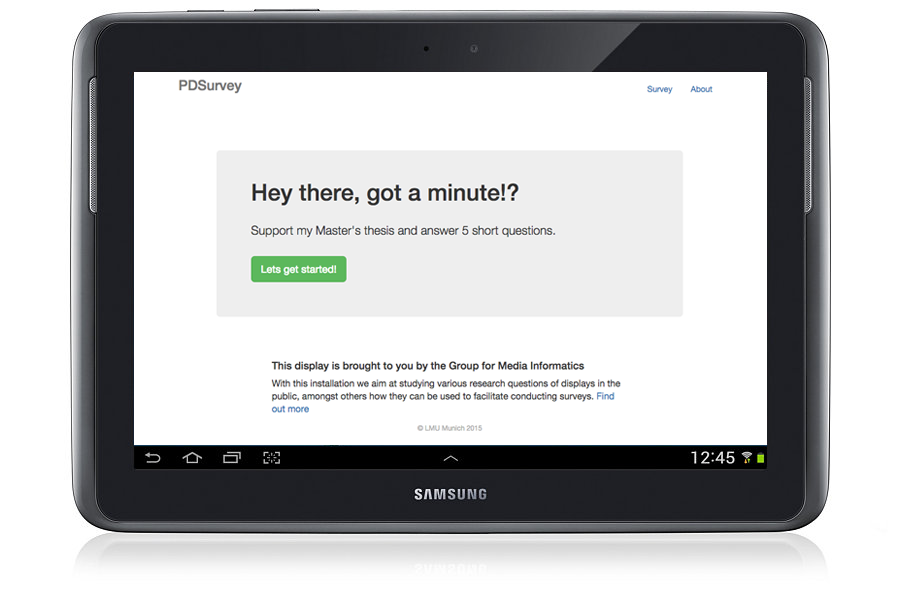
\includegraphics[width=.7\columnwidth]{img/5_field-study/pdclient-startscreen.png}
	    \end{center}
	 \caption{The Welcome Screen of PDClient, using intrinsic motivation to motivate users to participate in a short questionnaire.}
	 \label{fig:5-pdclient-intro}
	\end{figure}

	% Adjustments for Field Study / Intrinsic Motivation
	The days prior to the launch of the actual field study were used for assembly and for last adjustments, like change of font size, adjustment to the position of certain UI elements, and for collecting implicit feedback from users observing but not approaching the display. From only watching the people passing by, it could be seen that a more effective call-to-action was needed. Many people looked at the display and noticed that something had changed with the setup, but no one started interacting or was willing to complete the questionnaire. To increase the motivation for users to participate, the start screens were improved based on the findings of the self-determination theory introduced by Richard Ryan\footnote{http://www.selfdeterminationtheory.org/} \cite{ryan2000self}. We stated on the Welcome screen of the tablet (see figure \ref{fig:5-pdclient-intro}) and on the Options panel of the TV Screen (see figure \ref{fig:5-feedback-options}) that the questionnaire only consists of five questions, that it will only take one minute to complete and the results are for a Master's thesis at the university. This resulted in an increased response and acceptance rate of the survey.



	



% \clearpage
\subsection{Study}

	% give the reader enough information to replicate the experiment
	We deployed the \textit{PDSurvey} platform to a public display setup, which had already been running since several months in the entrance hall of the faculty building. The public display setup had consistently attracted new and returning users to participate. A descriptive research type was chosen as the study type. Our aim is to describe and observe how users react to the new display setup. Only one study prototype is deployed, without varying any variables. The goal was to get first feedback on how people perceive filling in questionnaires on digital signage in public, before getting into more fine-grained research (see chapter \ref{chapter:future-work}). 
	Both quantitative and qualitative data was collected as part of the field study. Quantitative data was obtained through the \textit{PDSurvey} system and qualitative data was collected through semi-structured interviews.
	The distribution of the preferred feedback channel was logged inside of the Balloon Shooter game (see section \ref{chapter:field-study:apparatus}) and asked in all semi-structured interviews.


	\subsubsection{Design}
	\label{chapter:field-study:design}

	% Goal: Which Feedback Channel
	Our primary goal was to find out which feedback channel users preferred to respond to surveys in public. Each user had the choice to respond to the questionnaire on a TV display (1), on a tablet (2) to the right of the TV screen, via their own smartphone (3) or via email (4). The order of all four feedback options was randomized.
	After completing the Balloon Shooter game on the primary TV screen, each participant was confronted with an options panel (see figure \ref{fig:5-feedback-options}), asking the user to support our research and to respond to a short questionnaire. The feedback channel chosen was logged and the user had the opportunity to respond to the same questionnaire on any of four feedback channels. 
	We displayed the same five questions (see table \ref{table:questions-asked}) and chose to limit the number to five questions, to avoid low participation rate and low response rate.

	\begin{figure}
	    \begin{center}
			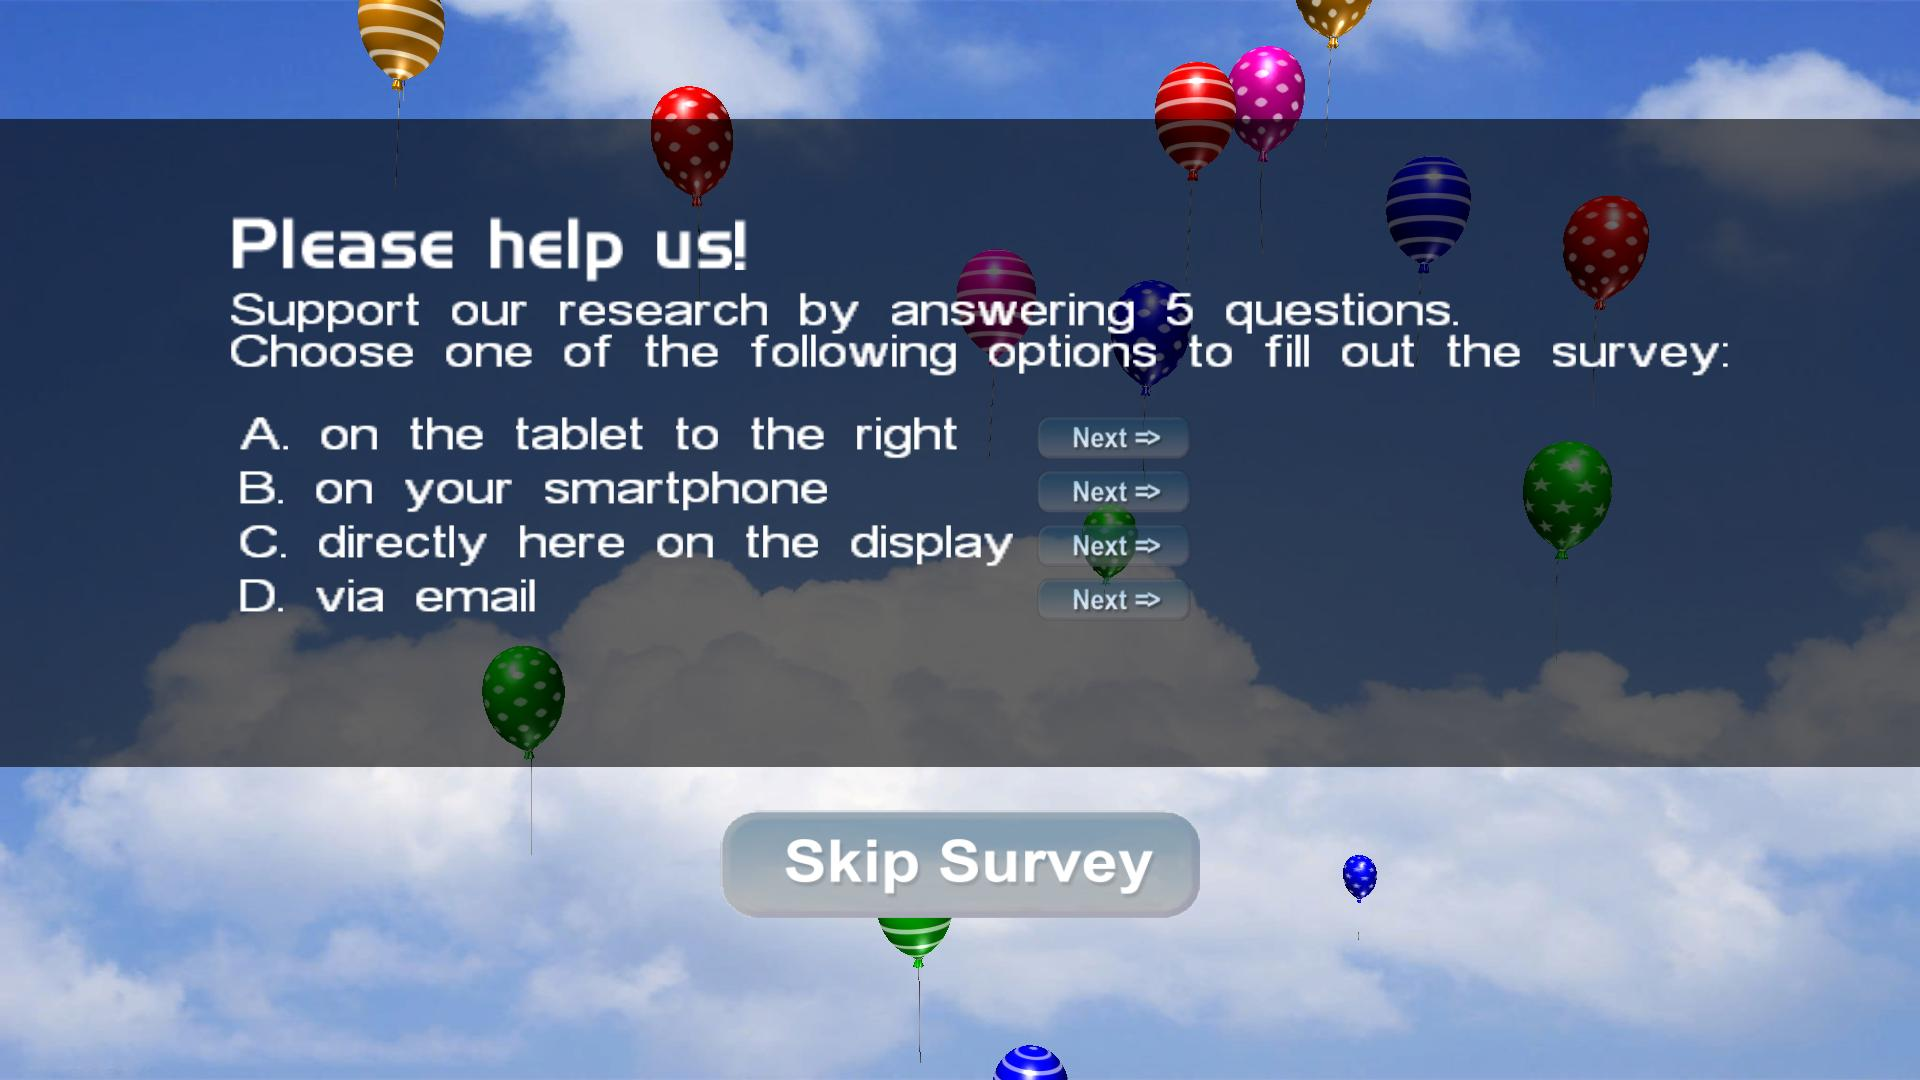
\includegraphics[width=.65\columnwidth]{img/screenshots/balloon-game/options-overview.jpg}
	    \end{center}
	 \caption[Feedback Channel: Options Panel]{Options panel, embedded after a game of Balloon Shooter, prompting the user to choose a feedback channel. Screenshot by Jiamin Shi.}
	 \label{fig:5-feedback-options}
	\end{figure}

	% Table: Questions asked on PDClient
	\begin{table}[bth]
		\small
		\center
		\begin{tabular}{lc}
\toprule
\textbf{Wording}                                                     & \textbf{Question Type} \\ \midrule
1. How often have you used this display before?                         & Numeric                \\
2. How likely is it that you will use this display in the future again? & 5-point Likert scale   \\
3. Which devices do you possess or use regularly?                       & Multiple choice, 5 options                        \\
4. In which area do you study / work?                                   & Text field             \\
5. What was your motivation for approaching and using this display?     & Text field            \\
\bottomrule
\end{tabular}

		\caption[Questions asked]{Questions asked on all four feedback channels}
		\label{table:questions-asked}
	\end{table}

	% I: QUESTIONNAIRE

	% Question Types
	In order to also get first insights into how well certain question types are suited for surveys in public, where a short completion time is crucial, we varied between the following question types and kept them in the same order: numeric questions, Likert scale, multiple choice (based on check boxes) and two text fields for responses of undefined length. 
	% Study setup: pure observation (no indep. variables / conditions)
	Due to the nature of descriptive studies, we only observed the users' behavior and observed how our study setup was used. The parameter of interest was the feedback channel chosen to respond to the survey. Since we didn't vary any conditions, no independent variables are present.
	% II: SEMI-STRUCTURED INTERVIEW
	To find out more about the users' motives for approaching the display setup, we also carried out semi-structured interviews in parallel to the field study of the PDSurvey platform. The goal of the interviews was to get qualitative feedback from all age groups and backgrounds. Getting a better understanding of how people respond to questionnaires in public, helps us improve the \textit{PDSurvey} platform.





	\subsubsection{Apparatus}
	\label{chapter:field-study:apparatus}
		% give details of any equipment used, including thinkgs like questionnaires and other tests

		The permanent setup consisted of a 55-inch touch-sensitive TV screen, connected to a laptop running on Windows 7, and a Samsung Galaxy Tab 10.1 tablet positioned to the right of the TV screen on a console. The TV screen was positioned on a 60cm high stand, resulting in a positioning at eye level. The tablet was placed on and fixed to a conductor's stand to the right of the TV screen (see figure \ref{fig:5-study-setup}). Our object of investigation was the TV screen with touch support, running an interactive game called \textit{Balloon Shooter}, developed by Jiamin Shi. After users completed the game, they were asked via a prompt to fill in a questionnaire on one of the four provided feedback channels (see figure \ref{fig:5-feedback-options}). The courtesy for the Balloon Shooter game and the survey implementation on the TV screen goes to Jiamin Shi.

		\begin{figure}
		    \begin{center}
   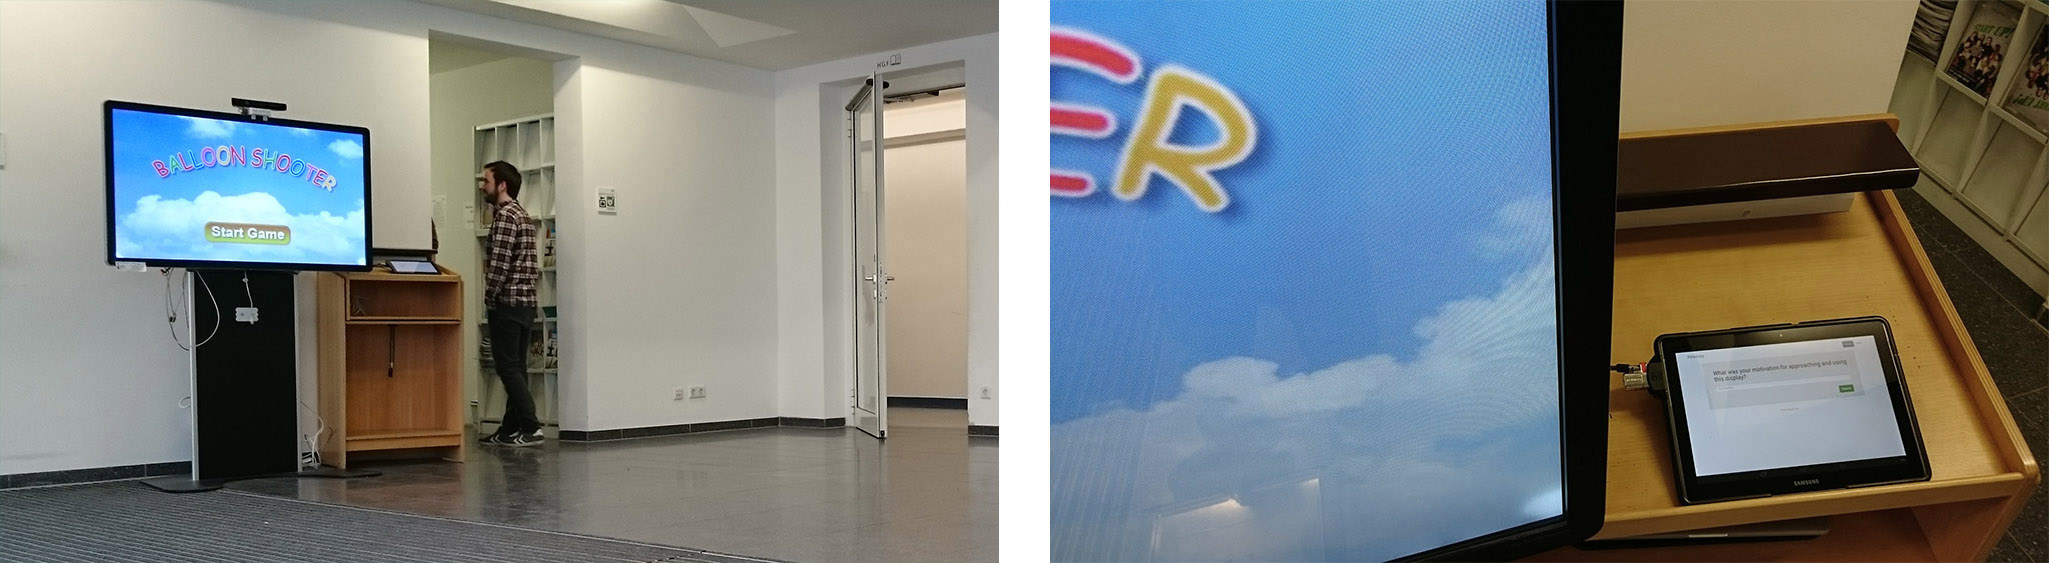
\includegraphics[width=\columnwidth]{img/5_field-study/study-setup.jpg}
		    \end{center}
		 \caption{Overview of the study setup in the entrance hall of the faculty building.}
		 \label{fig:5-study-setup}
		\end{figure}

		Each user had the opportunity to respond to the \textit{questionnaire} either directly on the TV screen (1), on the tablet to the right of the big TV (2), via their own smartphone (3) or via email (4). The first option was embedded natively into the Balloon Shooter game, offering a consistent UI and the most direct feedback channel. When choosing the tablet as an option, users were prompted to move to the right and to answer five questions on the tablet. The Android tablet was running KioWare Lite\footnote{\url{http://www.kioware.com/android.aspx} (last accessed on April 21, 2015)}, a kiosk app for Android, and displaying the responsive frontend of PDClient for the entire time of the study. Choosing the third option prompted the user to either scan a QR code with their smartphone or to open a URL\footnote{\url{https://pdsurvey.herokuapp.com/} (last accessed on April 21, 2015)} in their mobile browser. The last option consisted of an input field embedded into the Balloon Shooter game on the TV screen, asking the user to enter their email address. The address was logged to a txt-file, which was scanned every 5 minutes by the Windows task scheduler. An email reminder was sent to the user with a request to complete the survey. For sending the email from the TV screen, a Python script\footnote{\url{https://github.com/lukasziegler/python-send-mail} (accessed on March 15, 2015)} was written, using a modified version of TLS authentication in order to comply with the university's SMTP server. Screenshots of all four options can be found in Appendix \ref{appendix:screenshots-balloon-shooter} on page \pageref{appendix:screenshots-balloon-shooter}.
		% What was logged
		For the permanent setup the following data was logged: the timestamp of the users' choice, which feedback channel the user chose to respond to the survey, and whether they skipped the call to participate in the survey or if they stopped playing the game (determined via timeout). 
		% Questionnaire used
		On all four feedback channels a self-made questionnaire was used, since the focus was on finding which channels and question types are best suited in general for being used on public display. This was the reason why we did not use any of the standardized questionnaires mentioned in chapter \ref{chapter:literature-review}. 

		% II) SEMI STRUCTURED INTERVIEW
		For conducting the \textit{semi-structured interviews}, two questionnaires were used as a rough guide, one for participants, and one for passerby. A voice-recorder (smartphone) was used additionally to record the interviews, to be able transcribe and code all of conducted interviews. Each semi-structured interview loosely followed the outline presented on page \pageref{appendix:semi-structured-interview}. Audio recordings and transcriptions are on the attached CD.
		% III) BALLOON SHOOTER GAME
		The main application installed on the public display was a game called \textit{Balloon Shooter} developed and run by Jiamin Shi, a PhD student at the Group for Media Informatics at LMU Munich. It was first installed on January 7th 2015 and has been running in different versions since then. The public audience had already used it for roughly two months and had adapted to it well. In 2.5 weeks in February\footnote{Based on the evaluation of log data from 05/02/2015 to 23/02/2015, reported by Jiamin Shi.} usage statistics reported that the game was played a total of 305 times.



	\subsubsection{Location}

		All parts of the field study were carried out in Oettingenstrasse 67, the faculty building for Computer Science of Ludwig-Maximilians-Universit\"at M\"unchen. Research institutes for Ethnology, Political Science, Japanese Studies, and Physics are also located in the same building. The study was carried out in the entrance hall of the university building. Figure \ref{fig:5-entrance-hall} gives an overview of the entrance hall and of the paths most people take while crossing the room. The excerpt is based on the universities floor plan\footnote{\url{http://www.uni-muenchen.de/funktionen/gebaeudeplaene/7070_d_00.pdf} (last accessed on March 22, 2015)}, and was inspired by Sandra Zollner \cite{zollner2014thesis}. For her bachelor's thesis she conducted a study in the same location one year ago and analyzed the visitor flow. According to Zollner ``approximately 59\% of all passers-by used path 1'' to get something from the lockers or to leave through the door to the library. 28\% of the people were taking path 2 and 13\% were taking path 3.
		% My observations
		In our field study it was also evident that the majority of the visitors took path 1. This group usually was fairly target-orientated, or in a hurry. Otherwise, on days with bad weather, people had their break in the entrance hall, or waited for someone. On days with good weather people usually took their breaks outside and only passed through the entrance hall, coming from the library, picking up something from the locker room and going outside.

		\begin{figure}%[hb]
		    \begin{center}
		     \fbox{	
		     	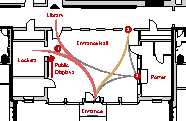
\includegraphics[width=.7\columnwidth]{img/5_field-study/entrance-hall.pdf}
		     }
		    \end{center}
			 \caption[Floor Map of Entrance Hall]{Floor map of the entrance hall, where the field study was carried out. User paths, and the surrounding environment including facilities such as the library can be seen.}
			 \label{fig:5-entrance-hall}
		\end{figure}




	\subsubsection{Procedure}
		% tell the reader how the study was carried out in practice

		All participants of the semi-structured interview were asked a similar set of questions (see Appendix \ref{appendix:interviews}). Based on the group they belonged to, either questionnaire 1 (for participants of the display setup) or questionnaire 2 (for passersby) was chosen. In order to speed up the interviewing process and to get away from a plain question-response schema, the questions on the printed out questionnaire only served as a rough guideline. 

		% Instructions given
		For people having trouble understanding the concept of the public display installation, the situation was described as follows. ``Imagine you are in a shopping mall or at an airport using one of those large displays to find some information. After finding what you were looking for, you are asked to answer a short questionnaire. How would you react to it?'' A full transcription of all questions and responses can also be found on the enclosed CD. 

		The participants for the PDSurvey questionnaire were not additionally motivated. All they saw was the options panel after completing the Balloon Shooter game (see figure \ref{fig:5-feedback-options}) or the welcome screen of the tablet (see figure \ref{fig:5-pdclient-intro}) while passing through the entrance hall. A complete copy of what the users were able to interact with, can be seen on the attached CD (see Appendix \ref{appendix:cd-contents}).







	\subsubsection{Participants} % provide the necessary information about the people who took part in your experiment
	\label{chapter:field-study:participants}

		In total 57 questionnaires were submitted and 28 semi-structured interviews were conducted during the two week study period. As for the study size, we took the findings from Alt et al.\cite{Alt2012HowToEvaluate} as a rough guide, for how many participants to include in our study. According to Alt et al. most field studies have an average of 26.9 interviews and 38.4 questionnaire responses. Information about the background of the participants was assessed both in the questionnaire and in semi-structured interviews (see table \ref{table:demographics}). Due to the limited number of questions in the questionnaire, only one the age of the participant was asked. In the semi-structured interviews information regarding the participants' age, gender, and working/study area were asked.

		Based on the fourth question (``In which area do you study / work?'') we can draw a conclusion about the study field of the survey participants. As far as indicated all people responding to the \textit{questionnaire} installed on the public display setup were students. Out of 57 responses, 42 could be assigned to a study field. The remaining 12 submissions consisted of responses such as \textit{bavaria, bib, home, munich, muc} or were left empty. The study fields most frequently represented were Computer Science (23.8\%), followed by Political Science (14.3\%), Japanese Studies (11.9\%), and Anthropology (11.9\%), Cultural Science (9.5\%), and Business (9.5\%). Other study fields mentioned were Physics, Sociology, Ethnology, Communication Science, Sports, and Science \& Technology. 

		For the \textit{semi-structured interviews} we collected more detailed information about the participants' backgrounds. Out of the 28 participants, 72.4\% were male and 28.6\% were female. The average age was 31 years, with an age distribution ranging from 20 years up to 69 years (median=25, SD=13.2). Due to the wide variety of faculties and a library being located in the same building, various technical backgrounds were present. What they all had in common was their affiliation to LMU Munich, either because of being a student themselves, working at the university or being otherwise connected to the university. In total 23 students, three employees, and two retirees were interviewed. The study fields which were most frequently represented are Computer Science (16.7\%), Japanese Studies (16.7\%), Ethnology (12.5\%), and Political Science (12.5\%). Other areas mentioned were Sociology, Communication Science, Law, Physics and Engineering. 
		% Participants vs Passer-by
		Eleven of the 28 interviews were conducted with actual participants of the public display study setup (39.3\%), the remaining 17 interviewees (60.7\%) consisted of people passing-by the display setup.


		\begin{table}%[bh]
			\small
			\center
			\begin{tabular}{lllll}
\toprule
   & \textbf{Participants Of Survey} &  &   & \textbf{People Interviewed}                        \\
   \midrule
10 & Informatics                            &  & 4 & Informatics                                        \\
6  & Political Science                      &  & 4 & Japanology                                         \\
5  & Japanese Studies                       &  & 3 & Ethnology                                          \\
5  & Anthropology                           &  & 3 & Political Science                                  \\
4  & Cultural Science                       &  & 3 & \textit{employees} (PhD, public officer, SysAdmin) \\
4  & Business                               &  & 2 & \textit{in pension}                                \\
2  & Physics                                &  & 1 & Communication Science                              \\
2  & Sociology                              &  & 1 & Sociology                                          \\
1  & Ethnology                              &  & 1 & Law                                                \\
1  & Communication Science                  &  & 1 & Physics                                            \\
1  & Sports                                 &  & 1 & Engineering                                        \\
1  & Science and Technology                 &  &   &               \\
\bottomrule
\end{tabular}

			\caption[Demographics of Field Study]{Demography for the survey data (left) and the semi-structured interview (right).}
			\label{table:demographics}
		\end{table}


		% HOW WE OBTAINED THE PARTICIPANTS
		The selection of participants for the completion of the \textit{questionnaire} was not influenced by us. All survey responses were made in their own interest and no reward was given for participating in this ``in the wild''-study. The selection of the participants for the \textit{semi-structured interviews} was influenced by how users reacted to the display setup. Our primary goal was to observe and interview active users of the public display setup, in order to get a better understanding of how they perceived the setup and to get insights into which feedback channel they chose and why they chose it. In order to also understand why people did not approach, or if they have any concerns, people passing by were also interviewed. 
		
		Before starting the semi-structured interviews, all people participating were asked whether they had already noticed the display setup and/or the option to fill in a survey. 
		This allowed us to consider the novelty effect for evaluation and to differentiate between three groups: participants who approached the display by themselves (and were observed doing so), people passing by the display (noticing the display, however not approaching it) and the last group of people simply passing by (not having noticed the display). The distribution between the groups was as follows: 11 active participants, 14 passerby (who had noticed the displays before), and 3 passerby (who saw the display setup for the first time). 

		Out of all people passing by no one has noticed the option to fill in a survey. Out of the active participants, 5 out of 11 have noticed the option to respond to a survey on different channels.
		To increase the amount of feedback, we approached people from all three groups. The number of survey responses was not artificially increased by asking passersby was.
		



		% REMINDER: only give RELEVANT information to the reader!
		% > only provide details if they are needed for replication
		% > or if they are relevant to the outcome of the experiment



\clearpage
\subsection{Results}

%%% QUANTITATIVE DATA %%% = pure facts
  % just tell the reader what you found

	We received a total of 57 filled in surveys, submitted via all four of the provided feedback channels, and carried out 28 semi-structured interviews. No treatments were applied to the dataset, descriptive statistics will follow below. The presentation of the evaluation is divided into three parts. First, we review which feedback channel is most popular, followed by the quantitative results of the PDSurvey questionnaire, and concluding with the results from the semi-structured interview. 


% I) Descriptive Statistics
% - provide summaries of group performance
% - present: average, mean, mode
% - describes: standard deviation, range (how it is spread)
% - describes: frequency of data (if relevant)

% presentation of data
% - don't present data multiple times
% - either use a TABLE or a GRAPH
% - always explain to the reader in words what the results show
% - tables / graphs should be self explanatory
% - the text should be comprehensible without taking a look at the figures




	\subsubsection{Feedback Channels}
	\label{5:results:feedback-channels}

	The preferred feedback channel was determined in three ways, first, based on the log file from the options panel of the TV screen (see figure \ref{fig:5-feedback-options}), second, based on the interview responses, and third, by analyzing all of the logged questionnaire responses made on all four feedback channels. The third way, however, has to be treated with caution, since it evaluates all logged responses, which is prone to distortions.

	% PREFERRED CHANNEL
	For the first way, users had the option to choose one of the four offered feedback channels through a selection on the large TV screen. Based on this log data of the TV screen, a good comparison of the feedback channels can be made, since all direct responses made on the tablet are excluded from this summary. The most popular feedback channel was the tablet (46.15\%), followed by the TV screen (30.77\%), smartphone (15.38\%), and email (7.69\%).
	% based on Interviews
	In order to have another source of input, the same question was asked at the end of every semi-structured interview. Based on this quantitative data from the interviews the response via tablet (42.86\%) was most popular again, followed by the TV screen (32.14\%). Interestingly, for the interview data the option to respond via email (17.86\%) is more popular than smartphone (7.14\%). 
	

	\begin{table}[h]

		% \begin{table}[h]
\center
\begin{tabular}{lllll}
\multicolumn{2}{l}{\textbf{From Survey Data}} &  & \multicolumn{2}{l}{\textbf{From Interviews}} \\
30.8\%                   & \multicolumn{3}{l}{on public display}      & 32.1\%                  \\
46.1\%                   & \multicolumn{3}{l}{on tablet}              & 42.9\%                  \\
15.4\%                   & \multicolumn{3}{l}{on smartphone}          & 7.1\%                   \\
7.7\%                    & \multicolumn{3}{l}{at home / via email}    & 17.9\%                 
\end{tabular}
\caption[Feedback Channel]{Preferred feedback channel for answering surveys.}
\label{table:5-feedback-channel}
\end{table}


	\parbox{.45\linewidth}{
		\centering
	    \begin{tabular}{ll}
	    \toprule
	    & Preferred feedback channelsl     \\
	    30.8\%       & on public display     \\
	    46.1\%       & on tablet         \\
	    15.4\%       &  on smartphone          \\
	    7.7\%        &  at home / via email        \\
	    \bottomrule
	    \end{tabular}   
		\caption{Based on survey responses}
	}
	\hfill
	\parbox{.45\linewidth}{
		\centering
	    \begin{tabular}{ll}
	    \toprule
	    32.1\%       & on public display     \\
	    42.9\%       & on tablet         \\
	    7.1\%       &  on smartphone          \\
	    17.9\%        &  at home / via email        \\
	    \bottomrule
	    \end{tabular} 
   		\caption{Based on interview questions}
	}


		\caption[Feedback Channel]{Preferred feedback channel for answering surveys.}
		\label{table:5-feedback-channel}
	\end{table}


	% LOG data / little bit distorted ...
	When evaluating all logged responses, the same sequence can be seen. The majority of the surveys were completed through the tablet, followed by the TV screen, smartphone, and email. The ratio, however, is highly distorted for this scenario. This is due to the tablets sole purpose being used to fill in surveys in our setup, and the additional intrinsic motivation given directly on the tablet's start screen (see section \ref{chapter:field-study:design}). The following ratio has to be treated with caution. In total 57 responses were made on all four feedback channels, 50 originated directly from the tablet (87.72\%). 4 responses were recorded on the TV screen (7.02\%), 2 via smartphone (3.51\%), and 1 via email (1.75\%). Since this listing only contains the number of responses, it should not be taken as a base for the comparison of the feedback channels' popularity. %% = interpretation! 
	For a comparison of the feedback channels the log data from the options panel and the responses of the semi-structured interviews are more suitable (see table \ref{table:5-feedback-channel}).




	\subsubsection{Survey Responses}
	\label{5:results:survey}
	%% Evaluation of all five questions

	Next is the evaluation of all responses made to the questionnaire. In total, 5 questions were asked on each feedback channel and 57 responses logged. Three times the response was canceled after the first question, once after the second question, four times after the third questions, the remaining 49 responses were complete.

	% 1) How OFTEN have the users USED this display BEFORE?
	The first question (\textit{How often have you used this display before?}) was measured as a numeric response. People have on average used the display 6.9 times before. For 25 people (43.9\% of the users) it was the first time using the display setup, 11 people (19.3\%) have used it once before, 18 people (31.6\%) between two and ten times, and the remaining 3 people (5.2\%) more than ten times.
	% 2) How LIKELY is it that you will USE THIS DEVICE AGAIN?
	For the second question (\textit{How likely is it that you will use this display in the future again?}), based on a 5-point Likert scale, the response was fairly uniformly distributed (average=3.04, SD=1.46). The whole scale from 1 (not likely at all) to 5 (very likely) was represented. No clear trend could be seen. When only considering the responses collected from the large TV screen, a clearer perception can be seen. There, the responses to this question had an average of 4.5 (SD=0.866), showing a trend towards a positive perception of the large display setup. However, due to the low number of responses for the TV display (only 4 responses), this conclusion cannot be regarded as significant. 
	% 3) DEVICES the users possess
	Taking a look at the devices users possess might give us first insights into why users chose which feedback channel (\textit{Which devices do you possess or use regularly?}). Overall, the majority of the people participating in the survey already owned a smartphone (79.3\%). The second most popular response was laptop (73.6\%), followed by tablet (41.5\%), and desktop computer (26.4\%). 18.9\% of the users indicated that they possess a feature phone and use it regularly. On average each participant possessed 2.4 devices. 
	When looking at which combinations of devices were most frequent, twelve people responded that they own a smartphone, tablet, and laptop. Twelve other people indicated that they possess a smartphone and laptop. Six people own a smartphone, laptop, and desktop.
	% 4) Study area >> demographics
	The fourth question (\textit{In which area do you study / work?}) was used to get a little insight into the background of the survey users. Only the occupation of each participant can be derived from the questionnaire. For a full evaluation of the demographic background of all participants, refer to section \ref{chapter:field-study:participants}.
	% 5) REASONS FOR APPROACHING
	The last question (\textit{What was your motivation for approaching and using this display?}) collected the main reasons why people have approached the display setup. The main reasons mentioned were ``curiosity'' (12x), ``fun'' (10x), ``boredom'' (8x), ``interest'' (2x), and ``during breaks'' (2x). Other reasons mentioned were ``it is there, so why not?'', ``it is there and colorful'', or ``I've never seen it before in this spot, wanted to know what it is about''.




	\subsubsection{Interview Responses}
	%% INTERVIEW DATA (a combination of facts + evaluation)

	The evaluation of the semi-structured interviews was based on Grounded Theory \cite{strauss1990basics}, promoting a systematic evaluation of the interview transcripts.
	% ANY INTERFERENCES
	To avoid any interferences between the two groups of people who have already participated in the study setup and people passing by, each passerby was asked, before starting the interview, whether he had noticed the public display setup, and whether he had already interacted with the installation. Out of all passersby no one had previously been interacted with the game or survey platform. 82.4\% (14 of 17) of the passersby had already noticed the public display installation before. However, none of the passersby had previously participated in the game. The remaining 17.6\% had neither approached the display nor noticed it prior to the interview. 


	% I) REASONS mentioned for choice of feedback channel
	% > TV Screen
	The semi-structured interview was most useful to get a better insight into why certain users chose which feedback channel. Reasons mentioned speaking for the \textit{TV screen} as the preferred choice were, because it is the ``most direct'' (4x) feedback option. Another popular reason was, because ``I am already standing here'' (2x). Reasons speaking against the TV screen for a lot of people are ``it is too large'' (4x), ``everyone could watch me'' (2x), and ``it feels too public'' (2x). 
	% > Tablet
	For the most popular feedback option, responding via \textit{tablet}, the following reasons speaking for the tablet were introduced: ``the display is smaller and better laid out'' (5x), ``better sensitivity / better usability'' (2x), ``it feels more private'' (2x), ``you are not in the way of others'', ``I am more used to it'', and ``less people are watching me''. Overall, only three people mentioned a reason speaking against the use of a tablet: ``redundancy'' (2x) and ``personal aversion''.
	% > Smartphone
	Two reasons, that were mentioned by participants of the semi-structured interview speaking for responding via their personal \textit{smartphone} were: ``it belongs to me'', and ``I use it most often''. Reasons why participants did not pick their smartphone, were more frequently: ``too much effort'' (4x), ``too indirect'' (3x), ``requires too much personal information'' (3x), ``I am not sure how complex and time-consuming it would be'' (2x).
	% > Email
	The last option, responding from elsewhere by submitting the \textit{email address}, turned out to be more popular than the previous option, responding via smartphone. Most people preferred this option due to the following reasons: ``I can do it at home'' (4x), ``I have more time to complete the survey'', and ``better warranty of privacy''. People would refrain from submitting their email address, because: ``I would forget about [responding]'' (5x), ``I don't like to submit my email address'' (4x), ``I don't like to postpone'' (3x), ``it would take too long to complete'' (2x), and it would be ``too much effort'' (2x). 
	For a full list of reasons mentioned for or against one of the feedback channels, refer to Appendix \ref{appendix:evaluation-of-PDs}.

	% Reasons for approaching
	From what has been mentioned, the main reason for approaching the public displays was ``curiosity'' (6x). Other reasons mentioned were ``for fun'', ``I was waiting for someone'', ``as a balance to studies'', ``I saw others using it'', and the novelty effect. Reasons for not approaching the display were ``no time'' (2x) and ``it is in the entry zone of the university, it feels strange when one plays with it'' (1x).
	%% III) ADDITIONAL OBSERVATIONS
	Additional observations made during the field study, are mentioned here briefly without comment.
	%% AGE Distribution per Feedback Channel
	When correlating the \textit{age distribution} per feedback channel, the following ratio can be seen. The highest age is on average on public display (31.6), followed by tablet (28.2), email (24.0) and smartphone (23.0).
	% response time
	The \textit{response time} for responding to the five questions was on average 1:02 minutes, ranging from 0:36 to 3:06 minutes.
	% number of acceptable questions
	The number of questions found acceptable on this setup ranged between five and ten questions.


	% II) OPEN CODING PHASE  >> exotic / unexpected responses
	The open coding phase of the Grounded Theory produced a few new aspects. What was to be expected, were the reasons speaking for and against each feedback channel, listed above. What wasn't predictable was that one person in his 50s preferred to use the large public display, due to his short-sightedness. In addition, one retired person refused to use any of the four offered digital feedback channels, even when being offered to be assisted by a person. This case should not be forgotten. Further, one participant was willing to provide her email address on the tablet, but not on the TV screen.
	% requirements for a survey
	Requirements stated, what the users would expect from a survey being conducted in public, are: ``it must be interesting on first sight'', ``it would help to see a benefit for oneself'', plus a ``good readability'' and `` understandability'' of the questions.

	

	%% TODO: VERGLEICHEN, ob es einen Unterschied gibt, zwischen den PARTICIPANTS und den PASSERSBY!!

	% >>> look at paper 29: great how they deconstructed their interviews and paraphrased all relevant data in a very compact way! <<<






\clearpage
\subsection{Discussion}
% here you tell them what it actually means for your research question
% for inspiration: http://www.ldeo.columbia.edu/~martins/sen_sem/thesis_org.html#Discussion


	% I) SUMMARY: a brief recapitulation
	In the field study we assessed which feedback channel users preferred, why users approached the display setup, and for which reason they made which choice. A vast majority of users preferred to respond directly in the public setting to the questionnaire. The tablet turned out to be the most popular feedback channel in the display setup, followed by the TV screen. Options email and smartphone accounted for only around a quarter of the total. Reasons for approaching the public displays were curiosity, novelty, for fun, mental balance, and pastime.

%The option email was chosen for better warranty of privacy, having more time and for a more private setting. The reasons stated for smartphone was chosen because of habit. 

	% II) Now allowing room for interpretation and personal opinions
	% > Feedback Channel
	It is interesting to see that the tablet is the most popular \textit{feedback channel} in all scenarios, although responding via the TV screen would be more a more direct approach and not require moving to another device. 
	Nevertheless all offered feedback channels were present in the evaluation and during the semi-structured interviews for each channel a good reason for the choice was given. What can be said is that our participants can be distinguished into three groups. The first (and slightly larger) group preferred the option of \textit{direct response}. They are not as concerned about answering questions in public and their privacy. For them it is more important to complete the survey as quickly as possible and not have to think about it later, as long as nothing too private or personal is asked. One person said ``If something too private would be asked, I would simply abort and go away from the display''. The second group is more concerned about \textit{privacy}. They are often of older age, or actually wanting to take the time to think about all of their responses in depth in order to give high-quality responses. This group prefers to take the questionnaire away from the public setting into their home. The third group chose the feedback channel purely based on their \textit{habit} and what they are accustomed to. Two women in their mid-twenties responded immediately ``on my smartphone, because I am most used to it''.
	These observations go along well with the five adaptation factors stated by Huang et al. \cite{Huang2004}: task specificity and deep integration, tool flexibility and generality, visibility and exposure to others' interaction, low barriers to use, dedicated core group of users.

	% > Display Size
	Another assumption we had made was encouraged by our observations and the semi-structured interviews: the smaller the display, the safer and more private the users feel. An exception to this finding could be old people. Once people's eye sight deteriorates with age or they get more insecure and uncertain with using new devices, they prefer to have a large input surface. But for the majority of younger people our assumption held true.
	% > Interaction Time
	Additionally, we made the observation that questionnaires on public displays are best suited for quantitative surveys. Users want a short interaction time, not having to think much about their answers and for roughly 25\% of the participants it holds true, that they do not like being observed while making responses in public.
	From this observation, the implication for the \textit{question types} can be derived: question types ideally with a single-click interaction are preferred (e.g. Likert scale, multiple choice with all options given, yes/no-questions). Followed by numeric, dropdown and multiple choice questions with one option for open-end responses. For these question types with a longer interaction time the user has to think a little bit more and assess more precisely to make a response. One example stated by a participant, in regards to the numeric question `\textit{How often have you used this display before?}', was that ``It would be great if you had the possibility to choose from a predefined range, because typing is not always optimal. I would prefer if areas would be given instead of oneself having to think about the exact number.'' Last, being no big surprise, are text fields combined with open-ended questions. As a take away for text fields: wherever possible rephrase the question so that the response can be as short as possible.

	% >> DRAWBACKS / FEARS

	What should not be forgotten are the fears mentioned during the qualitative evaluation. Concerns regarding loss of \textit{privacy}, and the increase of \textit{social desirability} in public settings. These are the two main constraints for surveys being conducted on displays in public settings, and should be taken into consideration when constructing new interactive display setups, which should offer the evaluation through a survey platform. Possible ways to cope with these concerns are to adjust the position of the display in public (not so exposed), and to vary the screen size depending on the required privacy.

% TODO >> wie man damit umgehen könnte...


	%% III) LIMITATIONS

	We are aware of certain limitations of our descriptive study. Our limitations are consistent with the findings found by Ojala et al. \cite{Ojala2011}. The effects of curiosity, impact of novelty, and influence of weather had an influence on our field study. Due to the novelty effect caused by the tablet, and the intrinsic motivation we added through the splash screen on the tablet (see section \ref{chapter:field-study:design}, self-determination theory), the participation rate on the tablet was increased. For our primary research question, which feedback channels is best suited, the impact of novelty, curiosity and of the always-visible tablet, should not have an impact. We based the evaluation of the feedback channel not on the overall number of responses, which was therefore distorted, but on the options panel and on the interview responses.
	Despite these effects, it was striking to see a response rate of 42.4\%, when comparing the 50 responses made on the tablet with the total number of 117 interactions made with the public display setup. When we exclude all participants who directly accessed the tablet and did not see the options panel to use one of the four feedback channels, the response rate on the tablet was still 5.1\%. 
	% Small future work section
	Otherwise, it should be mentioned that both the TV screen and the tablet were always on and that all questions were optional. One suggestion for improvement is to only turn on the screen of the tablet when it is selected on the TV screen as the desired feedback channel.

	% 4 DRAW CONCLUSION
	All in all, it can be said that people prefer to respond to questionnaires in public directly, as long as the questions don't get too private. Nonetheless the more feedback channels offered, the better it is, since the variety of user backgrounds also bring different preferences and attitudes. When designing public display setups for getting more private user input, the display size should also be taken into consideration. So far we have made the observation, that users feel more secure on smaller screens.
	% round off the discussion with some final conclusions
	For the development of our public display survey platform the study has shown that people of different age groups are willing to respond to questionnaires in public. 




%	\textbf{Concerns} that have been expressed: social desirability, less privacy. These concerns should be taken into consideration when designing questionnaires.

%	\textbf{Benefits being}: direct response, no procrastination, immediate feedback of the users impressions, less people needed for evaluation, semi-automated evaluation of the log data.



%  - - - - - - - - - - - - - - - - - - - - - 

% ggf. unterscheiden nach den drei Gruppen:
	% 1 participants who approached the display
	% 2 people passing by the display
	% 3 passing by, not having any intention to approach the display

% >> paper 25 for a good SAMPLE of how to list the basic population
% > paper #101 [CHI12BaillyShoeSense.pdf] "ShoeSense" contains another good evaluation